
\documentclass[tikz,border=8pt]{standalone}
\usepackage{amsmath}
\usetikzlibrary{arrows.meta,positioning}
\begin{document}
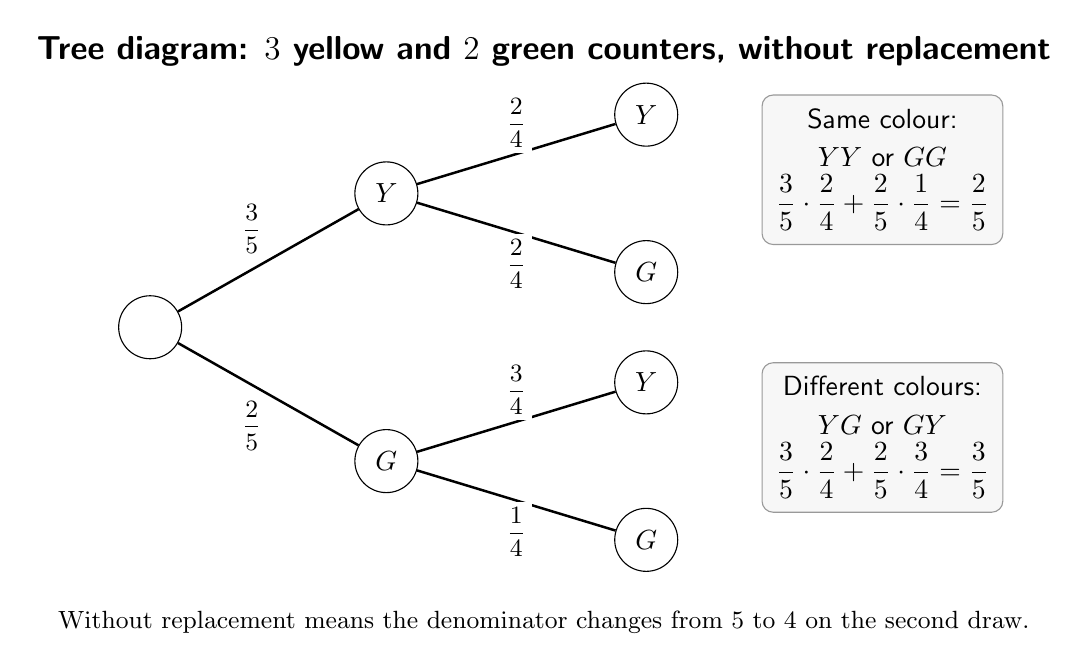
\begin{tikzpicture}[font=\sffamily,branch/.style={line width=0.9pt},outcome/.style={circle, draw=black, fill=white, minimum size=8mm, inner sep=0pt},prob/.style={midway, fill=white, inner sep=2pt, font=\small},note/.style={draw=black!40, rounded corners, fill=black!3, align=center, inner sep=5pt}]
\node[font=\sffamily\bfseries\large] at (5,3.5) {Tree diagram: $3$ yellow and $2$ green counters, without replacement};
\node[outcome] (start) at (0,0) {};\node[outcome] (Y1) at (3,1.7) {$Y$};\node[outcome] (G1) at (3,-1.7) {$G$};\node[outcome] (YY) at (6.3,2.7) {$Y$};\node[outcome] (YG) at (6.3,0.7) {$G$};\node[outcome] (GY) at (6.3,-0.7) {$Y$};\node[outcome] (GG) at (6.3,-2.7) {$G$};
\draw[branch] (start) -- (Y1) node[prob, above left] {$\dfrac{3}{5}$};\draw[branch] (start) -- (G1) node[prob, below left] {$\dfrac{2}{5}$};\draw[branch] (Y1) -- (YY) node[prob, above] {$\dfrac{2}{4}$};\draw[branch] (Y1) -- (YG) node[prob, below] {$\dfrac{2}{4}$};\draw[branch] (G1) -- (GY) node[prob, above] {$\dfrac{3}{4}$};\draw[branch] (G1) -- (GG) node[prob, below] {$\dfrac{1}{4}$};
\node[note] at (9.3,2.0) {Same colour:\\[2pt] $YY$ or $GG$\\[2pt] $\dfrac{3}{5}\cdot\dfrac{2}{4}+\dfrac{2}{5}\cdot\dfrac{1}{4}=\dfrac{2}{5}$};
\node[note] at (9.3,-1.4) {Different colours:\\[2pt] $YG$ or $GY$\\[2pt] $\dfrac{3}{5}\cdot\dfrac{2}{4}+\dfrac{2}{5}\cdot\dfrac{3}{4}=\dfrac{3}{5}$};
\node[align=center, font=\small] at (5,-3.75) {Without replacement means the denominator changes from $5$ to $4$ on the second draw.};
\end{tikzpicture}
\end{document}
